\documentclass[a4paper]{scrreprt}
\usepackage{fancyhdr}
\pagestyle{fancy}
\usepackage[english]{babel}
\usepackage[utf8]{inputenc}
\usepackage{graphicx}
\usepackage{url}
\usepackage{textcomp}
\usepackage{amsmath}
\usepackage{lastpage}
\usepackage{pgf}
\usepackage{wrapfig}
\usepackage{fancyvrb}
\usepackage{pdfpages}

\usepackage{etoolbox}
\makeatletter
\patchcmd{\scr@startchapter}{\if@openright\cleardoublepage\else\clearpage\fi}{}{}{}
\makeatother

% Create header and footer
\headheight 27pt
\pagestyle{fancyplain}
\lhead{\footnotesize{Applikationer för internet, ID1354}}
\chead{\footnotesize{Assignment 1 report}}
\rhead{}
\lfoot{}
\cfoot{\thepage\ (\pageref{LastPage})}
\rfoot{}

% Create title page
\title{Assignment 1}
\subtitle{Applikationer för internet, ID1354}
\author{Max Körlinge, korlinge@kth.se}
\date{\today}

\begin{document}

\maketitle

\tableofcontents %Generates the TOC
\clearpage

\chapter{Introduction}

This assignment concerns writing correct HTML and CSS for a website. You were instructed to create a website called "Tasty Recipes" according to certain specifications. All code was required to pass W3C validation, consider five basic heuristics for user interface design, and make sure the site behaves the same way on different browsers. Optional tasks were to make the site responsive and to take into account accessibility guidelines, which I did. I completed the task on my own.

\chapter{Literature Study}

To complete the task I studied the course lecture notes on HTML and CSS. I also read through the articles on heuristics for user interface design (which I found here:\\ https://www.nngroup.com/articles/ten-usability-heuristics/), and the accessibility guidelines referenced in the assignment (found here: https://www.w3.org/TR/WCAG10/).

\chapter{Method}

\section{Task 2}

Although the assignment stated that we could use finished online templates I decided to create my site by writing the bulk of the code myself. I have some experience with this although it's been a while since I wrote something from scratch and took this as an opportunity to learn.

By habit, developed from previous online learning material, I designed a mobile version first, since I knew I was going to make a responsive website. I coded the header and the navigation bar first to be able to copy it to the other pages, and then I coded the body of each specified page individually following the requirements. I use a popular reset CSS file called Normalize.css (https://necolas.github.io/normalize.css/) which is "A modern, HTML5-ready alternative to CSS resets".

After designing the mobile version of the website I step by step increased the resolution and added responsiveness to a sepearate CSS file responsive.css for different resolutions, for example putting the navigation bar to the left instead of below the header at a larger resolution.

For the calendar layout I used code from a github repository\\ (https://gist.github.com/starzonmyarmz/4496814). I used an article from CSS Tricks to help me design the layout using flexbox (https://css-tricks.com/snippets/css/a-guide-to-flexbox/).

For tooling I used VIM texteditor to write the code and the W3C Validator (https://validator.w3.org/) to validate it.

\section{Task 3}

I evaluated the site according to the explanations of the five heuristics found in the literature. The result can be found in the result chapter.

\section{Task 4}

I published my website on Github Pages (https://fongie.github.io) to use online tools for browser compability testing. It turned out that I couldnt find any that could test the Safari browser specified, and I do not a mac to install Safari on, so I had to skip it. I also couldn't find a single site to test all the desired browsers on, so I had to use a mix. I used browsershots.org to test firefox, a free trial on crossbrowsertesting.com to test chrome, and a local installation to test internet explorer.

\section{Optional Task 1}

See explanation in Task 2 (since I designed with responsiveness in mind from the start.)

\section{Optional Task 2}

To provide accessibility I first used alt tags for all img elements. 

I then scanned the site for places where there was no explanatory text or colors were used to indicate usage. On the index page I added a button clearly stating what clicking in the middle would do (take you to see the "recipe of the day", on the calendar).

I used the W3C validator to validate that I was using HTML and CSS properly and followed the validator's recommendations where it had any.


\chapter{Result}
\label{sec:result}

\section{Task 2}

The website can be found at https://fongie.github.io (currently, not permanently) and the git repository can be found at https://github.com/fongie/TastyRecipes.
The site contains the parts specified in the assignment: a welcoming home page (Fig. \ref{fig:design}), a calendar page with two recipes, and a page each for the recipes themselves.

\begin{figure}[h!]
  \begin{center}
    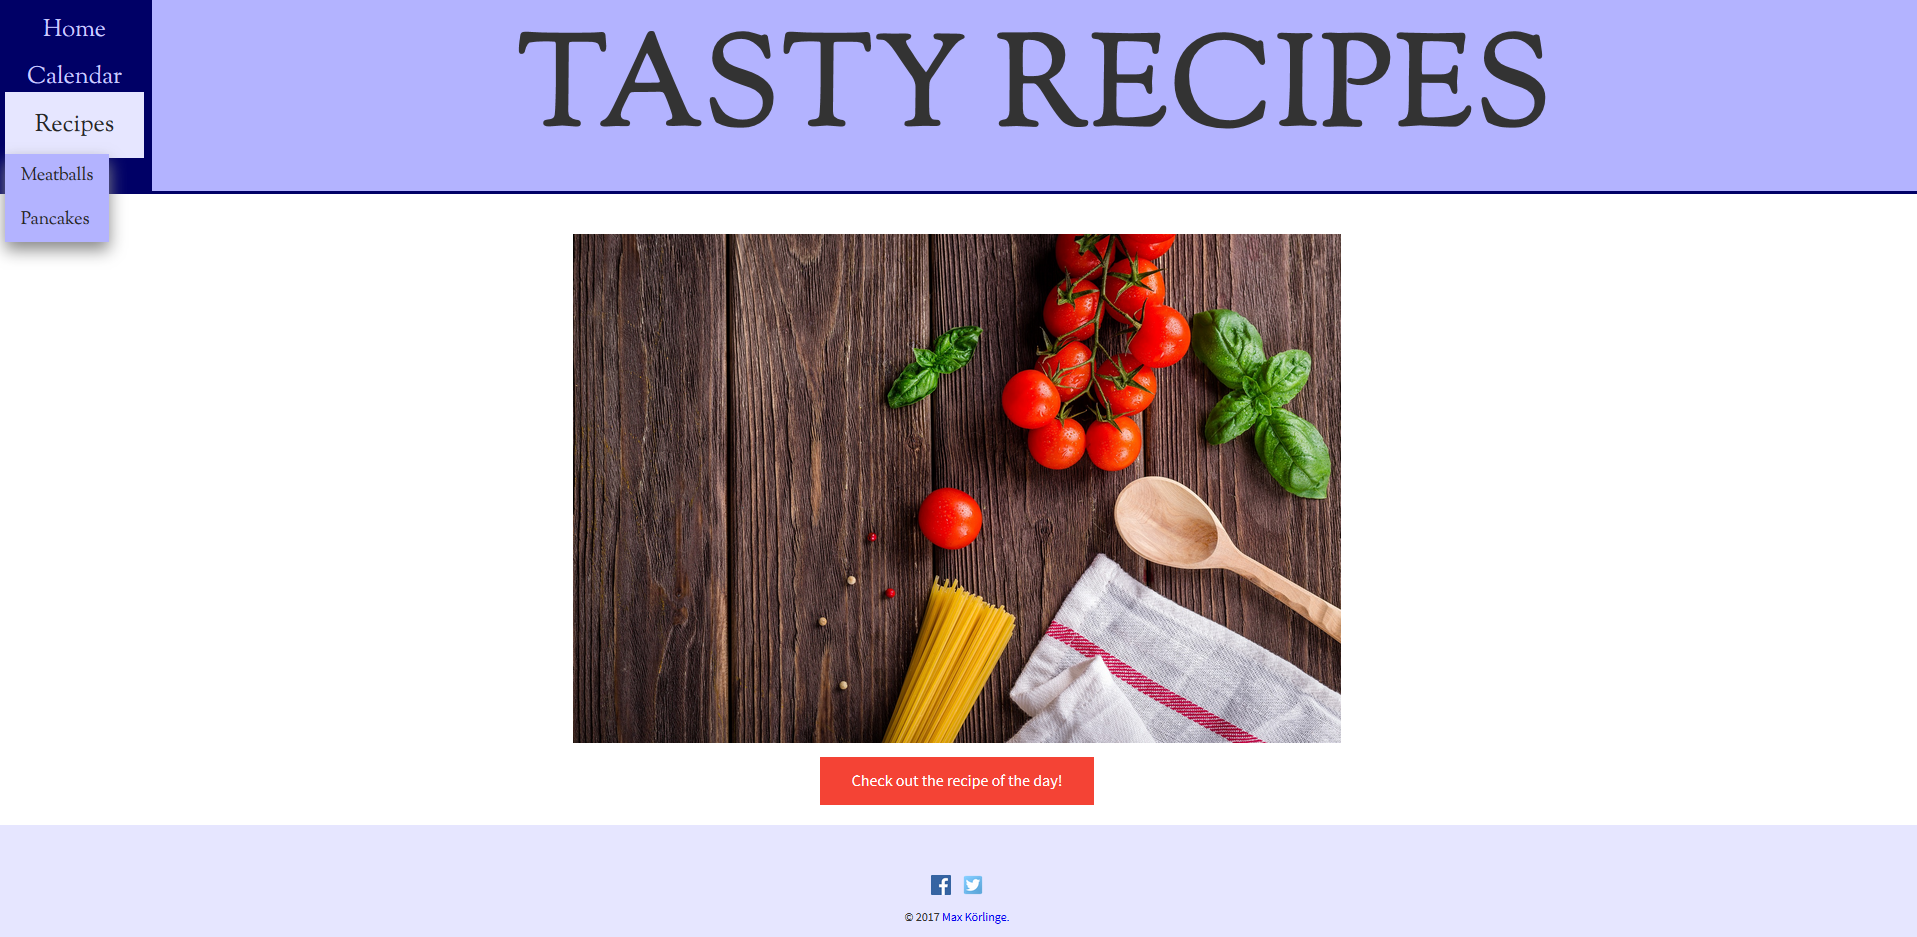
\includegraphics[scale=0.41]{design.png}
    \caption{The index page, showing navbar hover.}
    \label{fig:design}
  \end{center}
\end{figure}

All files passed the W3C validation, as shown in Figure \ref{fig:htmlvalidations} and \ref{fig:cssvalidations}. The files were also tested individually, as opposed to providing just the URL.

\begin{figure}[h!]
  \begin{center}
    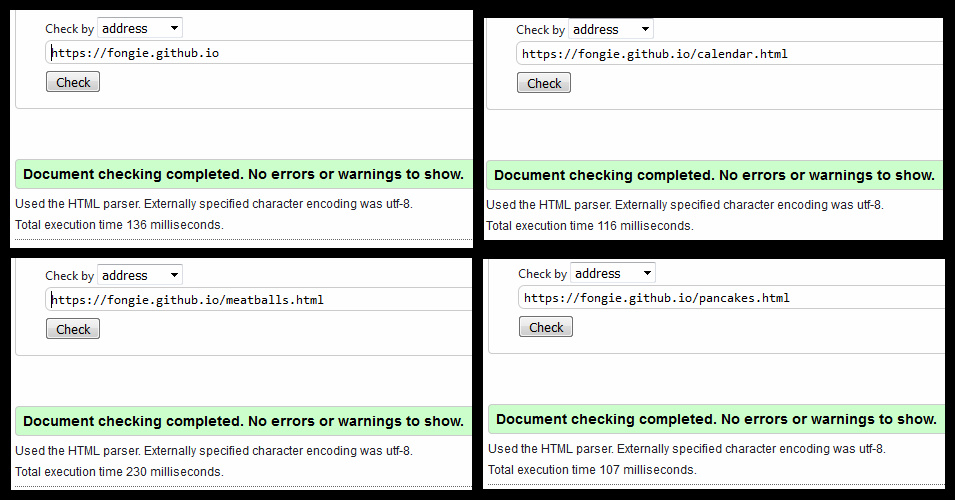
\includegraphics[scale=0.41]{htmlval/html_checks.jpeg}
    \caption{All W3C html validations.}
    \label{fig:htmlvalidations}
  \end{center}
\end{figure}

\begin{figure}[h!]
  \begin{center}
    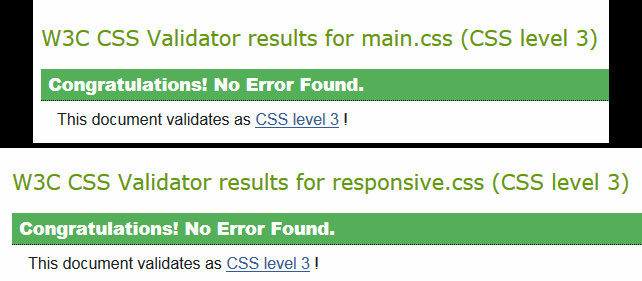
\includegraphics[scale=0.41]{cssval/css_checks.jpeg}
    \caption{All W3C css validations.}
    \label{fig:cssvalidations}
  \end{center}
\end{figure}


\section{Task 3}

Visibility of system status was considered but not found applicable for the site. Currently the site is completely static and does not have anything going on other than moving between static pages, so no loading or new elements appearing on the same site, and thus there is no real system status that needs to be shown to the user. Later I imagine there will be, when user will be able to post comments for example, the user would need to be told if the comment is being posted, failed to be posted, or was successfully posted.

A match between system and real world was sought after by not using any technical terms. The index page is called "Home", and in general there are normal, non-technical, words used throughout the site.

When it comes to consistency and standards the layout is fairly conventional as the navigation can be found somewhere at the top and in a bar of some sort. Also, all links are clearly displayed as buttons or images and the "pointer" cursor is used when hovering over links.

Recognition rather than recall is maintained mainly by the navbar, since all pages are always accessible through the navbar there is no need for the user to memorize how they got somewhere on the site.

The design is aestethic and minimalistic, using a sparse color palette of white and blue with only one alert-type red button. There is no eccess images or text floating about that do not add to the content or usability of the site. You are always only one or two clicks away from a recipe, and when arriving at the recipe you only have a picture of the food and bulleted lists of ingredients and how to make it.

\section{Task 4}

Although I unfortunately could not test Safari 9 I did test the others and it appears to be the same. I chose to display the Calendar page here since I think it might be the one that has the most complex css that could prevent compatibility, see Figure \ref{fig:compcheck}. Since I used different tools it was not possible to get them all at the same resolutions, but it is clear that they appear the same in all browsers nevertheless.

\begin{figure}[h!]
  \begin{center}
    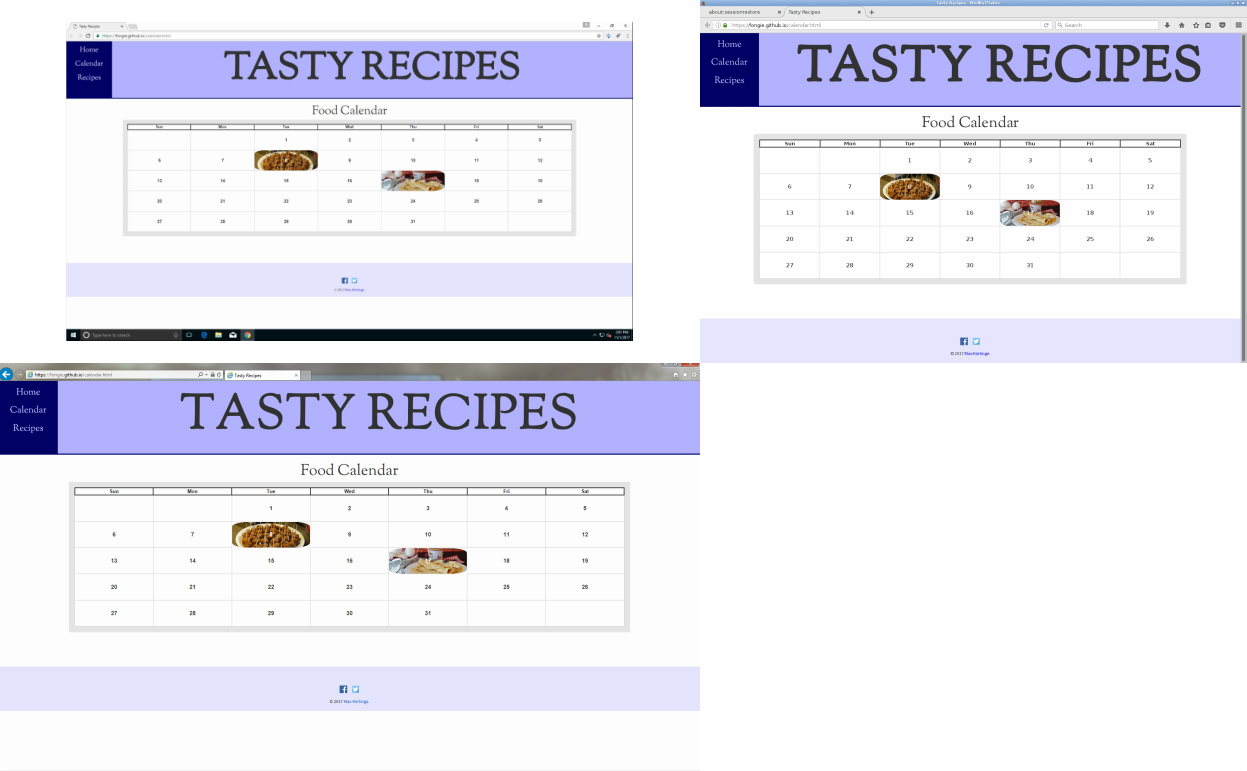
\includegraphics[scale=0.41]{compatability_check.jpg}
    \caption{Top left: Chrome 55, Top Right: Firefox 50, Bottom left: IE 10}
    \label{fig:compcheck}
  \end{center}
\end{figure}

\section{Optional Task 1}

The site was actually first designed for small resolution and later expanded to larger resolutions, by for example making some fonts larger, some images take less proportion of the screen, and moving the navbar to the left of the header. You can see the full size in Figure \ref{fig:design}, and the mobile version in Figure \ref{fig:mobversion}.

\begin{figure}[h!]
  \begin{center}
    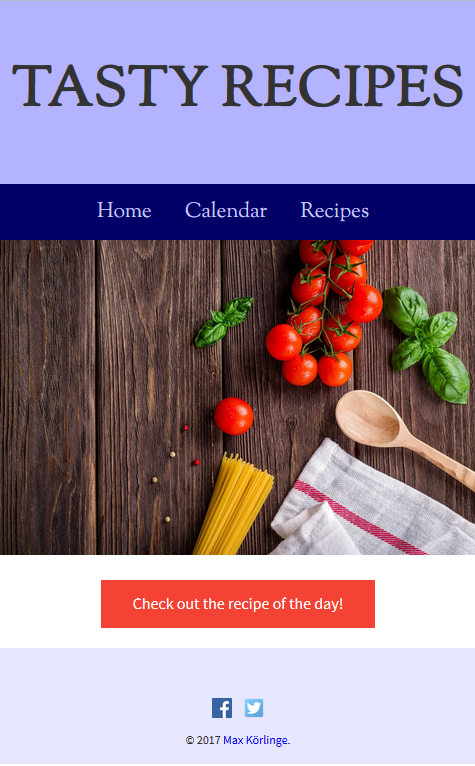
\includegraphics[scale=0.41]{mobversion.png}
    \caption{The mobile version.}
    \label{fig:mobversion}
  \end{center}
\end{figure}

\section{Optional Task 2}

The site has alt texts for all images and does not rely on color for example for highlighting things. When hovering over the calendar for example, it does not show where you are by changing color, but instead by giving the current cell a shadow which makes the cell "pop". As shown above all HTML and CSS was validated and thus used properly, and also as discussed previously, the navbar provides clear navigation mechanisms by always being present at a predictable place, and having links to all available pages.

\chapter{Discussion}

The task was to create a website according to certain specifications and which valides to proper HTML and CSS, a website which is responsive, accessible, compatible for different browsers, and minimalistic. In general I think the demands have been met. A few of the requirements were hard to apply to the site since it is so small and simple so far, like for example the UX criteria for visibility of system status. I also could not test one of the required browsers.

The design of the website and the general aesthetic look could be improved by using an online template, or by using for example Bootstrap for finished css classes, but I believe the look is acceptable, and most importantly, it is easy to navigate and use the site for its purpose.

The hardest part was trying to understand what the heuristics for user design and the accessibility guidelines concretely mean in terms of actual code. I think perhaps these are areas I can improve upon even though I have considered and tried to apply each one to the website as far as I understand them.

\chapter{Comments About the Course}

This is a fun and practical assignment. I found the required browsers to check really hard to find on any online tool, which was a little frustrating.

I spent about 15 hours on this assignment.


\end{document}
